\Testart{Skript}
\Titel{Objektorientierte Programmierung mit Java}

\large

\Hefteintrag{1.7}{Programmieren: Sprachen}{
Beim Programmieren schreibt man präzise und unmissverständliche Befehle, die dann vom \LoesungLuecke{Compiler}{6cm}~in Maschinensprache übersetzt werden. 

Hierfür gibt es verschiedene Programmiersprachen mit jeweils einer festgelegte \emphColA{Grammatik und Rechtschreibung (=\LoesungLuecke{Syntax}{4cm})}. Dem gegenüber steht die \emphColC{Logik eines Programms (=~\LoesungLuecke{Semantik}{4cm})}, die weitgehend unabhängig von der Programmiersprache ist.

\vspace{0.2cm}
Bei den einsteigerfreundlichen \emphColA{block-basierten Sprachen wie Blockly oder Online-Karol} übernehmen die Blöcke und ihre Verbindungsmöglichkeiten weitgehend die Einhaltung des Syntax. Bei \emphColC{text-basierten Sprachen wie \LoesungLuecke{Java}{6cm}~oder \LoesungLuecke{Python}{6cm}} müssen die Entwickler:innen selbst auf deren Einhaltung achten. Diese Sprachen bieten dadurch aber auch weitaus mehr Möglichkeiten (\emph{man sagt auch: sie sind mächtiger}). 

Dieses Skript arbeitet parallel mit den blockbasierten Sprachen Blockly und Online-Karol und der weit verbreiteten text-basierten und \emphColA{objektorientierten} Sprache \emphColA{Java}.

}


\begin{center}
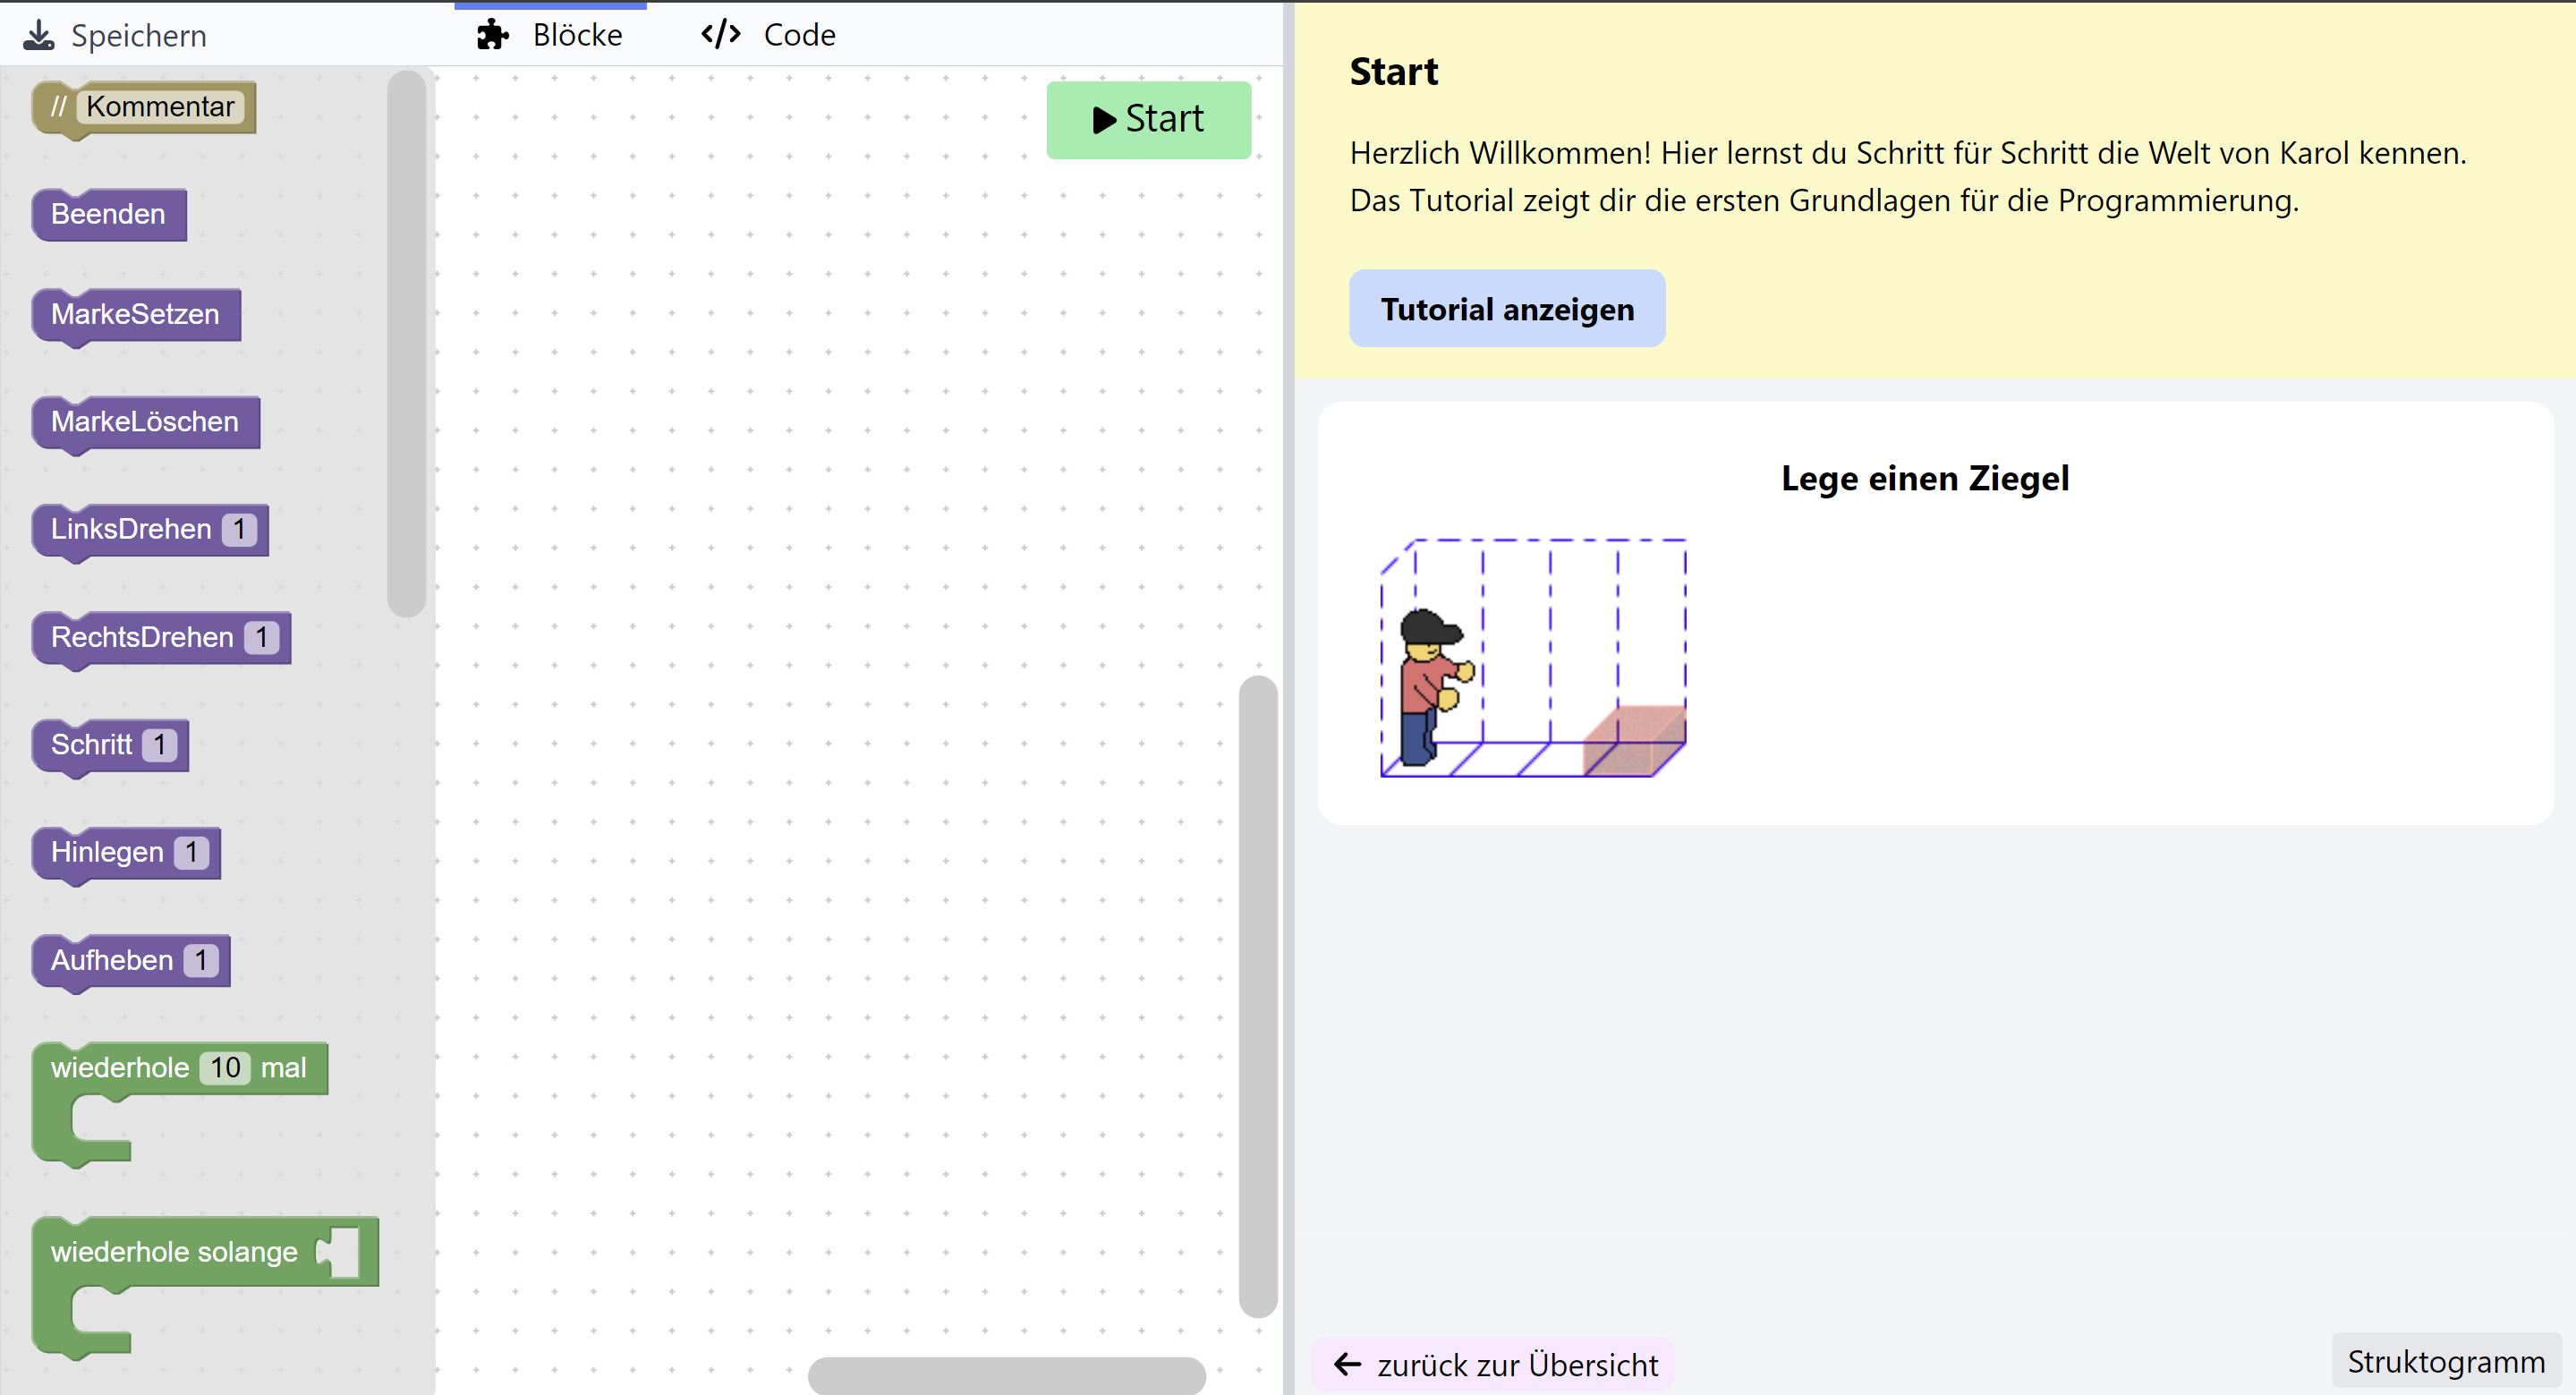
\includegraphics[width=0.85\textwidth]{_Aufgaben/BlocksAndJava/img/overview.png}
\end{center}

\Aufgabe{Karol-Java Übersetzung}{

\begin{enumerate}
    \item Bearbeite die Aufgaben von Robot Karol online: \url{karol.arrrg.de}
    \item Schalte in der Code-Ansicht die Sprache auf Java um und notiere auf dem AB jeweils zu welchem Java-Code der Block übersetzt wird. Achte hierbei auf Einrückungen!
\end{enumerate}


\begin{tabularx}{\textwidth}{p{4cm}X}


\includegraphics[height=25pt]{_Aufgaben/BlocksAndJava/img/step2.png}& \LoesungLine{karol.schritt(2);}{1}\\


\includegraphics[height=25pt]{_Aufgaben/BlocksAndJava/img/markeSetzen.png}& \LoesungLine{karol.markeSetzen();}{1}\\


\includegraphics[height=25pt]{_Aufgaben/BlocksAndJava/img/step10.png}& \LoesungLine{karol.schritt(10);}{1}\\

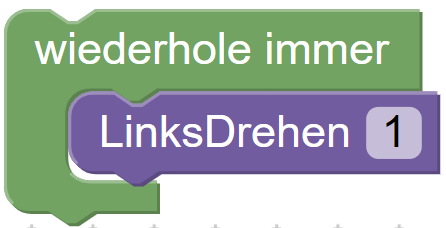
\includegraphics[width=\linewidth]{_Aufgaben/BlocksAndJava/img/whileTrue.png}&
\LoesungLine{while(true) \{ \newline \indent\hspace{1cm} karol.linksDrehen(1); \newline \} }{3}\\

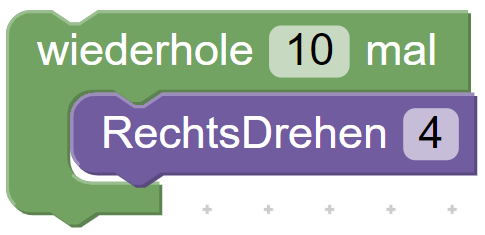
\includegraphics[width=\linewidth]{_Aufgaben/BlocksAndJava/img/for10.png}&\LoesungLine{for(int i=0; i < 10; i++) \{ \newline \indent\hspace{1cm} karol.rechtsDrehen(4); \newline \} }{3}

\end{tabularx}

\begin{tabularx}{\textwidth}{p{6cm}X}

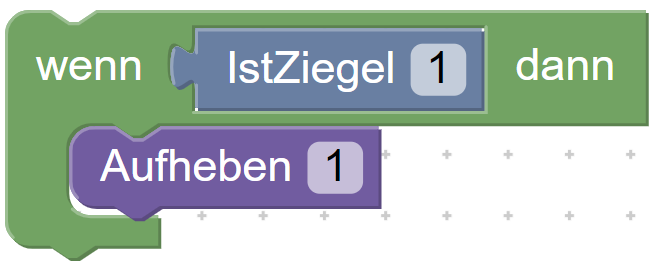
\includegraphics[width=\linewidth]{_Aufgaben/BlocksAndJava/img/if.png}& 
\LoesungLine{if(karol.istZiegel()) \{ \newline \indent\hspace{1cm} karol.aufheben(1); \newline \}}{3}\\\\

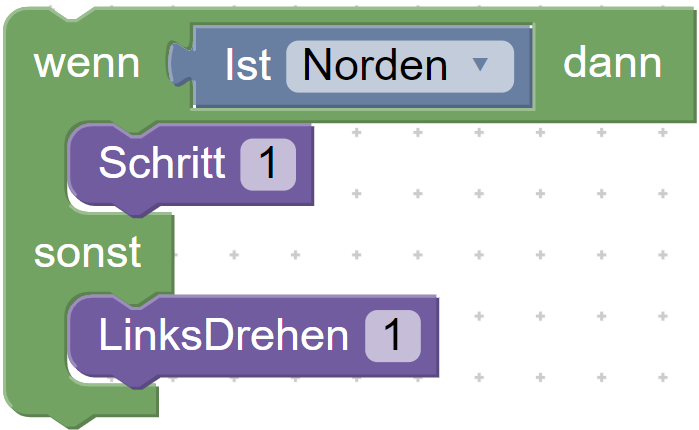
\includegraphics[width=\linewidth]{_Aufgaben/BlocksAndJava/img/ifelse.png}&
\LoesungLine{if(karol.istNordern()) \{ \newline \indent\hspace{1cm} karol.aufheben(1); \newline \} else \{ \newline \indent\hspace{1cm} karol.linksDrehen(1); \newline \}}{5}

\end{tabularx}

}


\Hefteintrag{1.2}{Übersicht Befehlsarten}{
\label{sec:befehlsarten}

Es gibt viele verschiedene Befehlsarten. Die für uns wichtigsten sind:

\begin{tabularx}{\textwidth}{b{0.5cm}>{\centering\arraybackslash}b{3.5cm}>{\centering\arraybackslash}b{3.5cm}>{\centering\arraybackslash}X>{\centering\arraybackslash}X}
\emphColA{Art}
& \emphColA{Online-Karol} 
& \emphColA{Blockly} 
& \emphColA{Java} 
& \emphColA{Struktogramm} \\ 

%\rotatebox{90}{\Loesung{einf. Befehl\color{black}}{\lineheight}}

\LoesungLeer{\multicolumn{5}{l}{\color{blue} einf. Befehl\color{black}}\\}
%

&
\includegraphics[width=\linewidth]{_Aufgaben//BlocklyJava_Skript//img/H02_karol_command.png}
&
\includegraphics[width=\linewidth]{_Aufgaben//BlocklyJava_Skript//img/H02_blockly_command.png}
&\LoesungKaro{karol.linksDrehen(1);\newline System.out.println("abc");}{4}
&\LoesungKaro{}{4}\\

\Loesung{\multicolumn{5}{l}{\color{blue} Verzweigung\color{black}}\\}

%\rotatebox{90}{\LoesungLine{Verzweigung}{1}}
&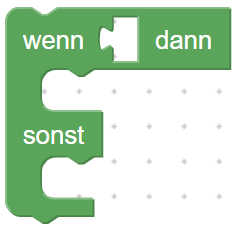
\includegraphics[width=\linewidth]{_Aufgaben//BlocklyJava_Skript//img/H02_karol_if-else.png}
&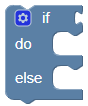
\includegraphics[width=2.5cm]{_Aufgaben//BlocklyJava_Skript//img/H02_blockly_if-else.png}
&\LoesungKaro{if(<Bedingung>) \{ \newline \indent\hspace{1cm} // wenn \newline \} else \{ \newline \indent\hspace{1cm} // sonst \newline \}}{7}
&\LoesungKaro{}{7}\\


\Loesung{\\\multicolumn{5}{l}{\color{blue} Schleife / bedingte Wiederholung\color{black}}\\}

%\rotatebox{90}{\LoesungLine{Schleife}{1}}
&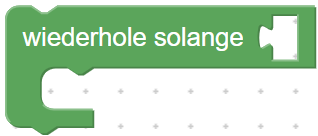
\includegraphics[width=\linewidth]{_Aufgaben//BlocklyJava_Skript//img/H02_karol_while.png}
&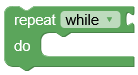
\includegraphics[width=\linewidth]{_Aufgaben//BlocklyJava_Skript//img/H02_blockly_while.png}
&\LoesungKaro{while(<Bedingung>) \{\newline...\newline\}}{5}
&\LoesungKaro{}{5}\\

\Loesung{\multicolumn{5}{l}{\color{blue} Zählschleife\color{black}}\\}

%\rotatebox{90}{\LoesungLine{Zählschleife}{1}}
&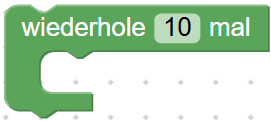
\includegraphics[width=\linewidth]{_Aufgaben//BlocklyJava_Skript//img/H02_karol_for.png}
&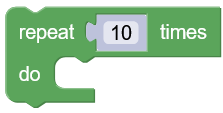
\includegraphics[width=\linewidth]{_Aufgaben//BlocklyJava_Skript//img/H02_blockly_for.png}
&\LoesungKaro{for(int i=0; i<10; i++) \{\newline...\newline\}}{7}
&\LoesungKaro{}{7}\\

\Loesung{\multicolumn{5}{l}{\color{blue} Methodendeklaration\color{black}}\\}

%\rotatebox{90}{\LoesungLine{M-Deklaration}{1}}
&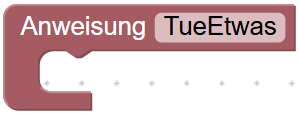
\includegraphics[width=\linewidth]{_Aufgaben//BlocklyJava_Skript//img/H02_karol_funcdef.png}
&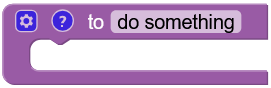
\includegraphics[width=\linewidth]{_Aufgaben//BlocklyJava_Skript//img/H02_blockly_funcdef.png}
&\LoesungKaro{public void doSomething() \{\newline...\newline\}}{5}
&\LoesungKaro{}{5}\\

\Loesung{\multicolumn{5}{l}{\color{blue} Methodenaufruf\color{black}}\\}

%\rotatebox{90}{\LoesungLine{M-Aufruf}{1}}
&
\includegraphics[width=\linewidth]{_Aufgaben//BlocklyJava_Skript//img/H02_karol_funccall.png}
&
\includegraphics[width=\linewidth]{_Aufgaben//BlocklyJava_Skript//img/H02_blockly_funccall.png}
&\LoesungKaro{doSomething();}{2}
&\LoesungKaro{}{2}\\

\Loesung{\\\multicolumn{5}{l}{\color{blue} Kommentar\color{black}}\\}

%\rotatebox{90}{\LoesungLine{Kommentar}{1}}
&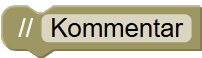
\includegraphics[width=\linewidth]{_Aufgaben//BlocklyJava_Skript//img/H02_karol_kommentar.png}
&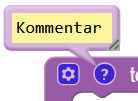
\includegraphics[width=0.8\linewidth]{_Aufgaben//BlocklyJava_Skript//img/H02_blockly_kommentar.png}
&\LoesungKaro{// Kommentar}{3}
&\LoesungKaro{}{3}\\


\Loesung{\\\multicolumn{5}{l}{\color{blue} Konstruktor\color{black}}\\}

%\rotatebox{90}{\LoesungLine{Konstruktor}{1}}
&%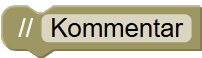
\includegraphics[width=\linewidth]{_Aufgaben//BlocklyJava_Skript//img/H02_karol_kommentar.png}
&
\includegraphics[width=1.1\linewidth]{_Aufgaben//BlocklyJava_Skript//img/H02_blockly_ctrdef.png}
&\LoesungKaro{public MeineKlasse() \{\newline...\newline\}}{4}
&\LoesungKaro{}{4}\\


\Loesung{\multicolumn{5}{l}{\color{blue} Objekt erstellen\color{black}}\\}

%\rotatebox{90}{\LoesungLine{Objekt erstellen}{1}}
%&%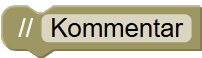
\includegraphics[width=\linewidth]{_Aufgaben//BlocklyJava_Skript//img/H02_karol_kommentar.png}
&
&
\includegraphics[width=1.1\linewidth]{_Aufgaben//BlocklyJava_Skript//img/H02_blockly_ctrcall.png}
&\LoesungKaro{new MeineKlasse();}{2}
&\LoesungKaro{}{2}\\

\end{tabularx}

}

\Aufgabe{Semikolon und geschweifte Klammern}

Wann macht man in Java ein Semikolon und wann setzt man geschweifte Klammern ein?

\begin{enumerate}
    \item Überlege zuerst allein (2 Minuten)
    \item Besprecht eure Überlegungen zu zweit und probiert sie in Online-Karol zur bestätigen (4 Minuten)
\end{enumerate}


\Hefteintrag{1.7}{Strukturierung von Programmcode - Syntax}{

In Java wird Programmcode vor allem mit \emphColA{\LoesungLuecke{Semikolons und geschweiften Klammern}{10cm}} strukturiert:

\doppelseite{0.55}{0.4}{t}{%
\begin{itemize}
    \item \LoesungLuecke{Semikolons}{5cm}~markieren das Ende eines \emphColA{einfachen Befehls oder Methodenaufrufs} (normalerweise am Ende der Zeile).
    \item \LoesungLuecke{Geschweifte Klammern}{7cm}~markieren \emphColA{Code-Abschnitte}, die wiederholt (Schleifen) oder bedingt (Bedingung) ausgeführt werden. Außerdem markieren sie den Methodenrumpf und Anfang und Ende einer Klasse. Je nachdem, was durch die Klammern markiert wird, spricht man synonym zu \LoesungLuecke{innerhalb}{5cm}~der Klammern auch von \LoesungLuecke{innerhalb}{5cm}~der Klasse, Methode, Schleife, etc.
\end{itemize}
}{%
\centering

\includegraphics[width=\linewidth]{_Aufgaben/BlocklyJava_Skript/img/H03_semicolonMeme.png}
\scriptsize www.reddit.com/r/ProgrammerHumor/comments/o0anud/semicolon}
}


\Hefteintrag{2}{Strukturierung von Programmcode - Semantik: Methoden}{%

Beim Programmieren können eigene Anweisungen/ Befehle/ Methoden/ Funktionen \textbf{deklariert} werden. Bei der \textbf{Deklaration beschreibt} zunächst mit dem \LoesungLuecke{Methodenkopf}{6cm}, welche Eigenschaften die Methode hat und anschließend im \LoesungLuecke{Methodenrumpf}{6cm}, wie genau sie sich verhalten soll. Eine deklarierte Methode kann anschließend beliebig oft verwendet (=\emphColA{aufgerufen}) werden.

Hierdurch kann man sehr lange Programme in übersichtlichere Einzelteile zerlegen, sodass \LoesungLuecke{doppelter Code}{8cm}~reduziert wird, der Code durch aussagekräftige \LoesungLuecke{Methodennamen}{6cm}~besser verstanden werden kann und Fehler schneller gefunden werden.

In Java darf außerdem kein auszuführender Programmcode außerhalb von Methoden sein.

Die Deklaration besteht aus \emphColB{Methodenkopf} und \emphColC{Methodenrumpf} (von geschweiften Klammern umschlossen):

{\ttfamily
\emphColB{void tueEtwas()} \emphColC{\{}

~~~~\emphColC{karol.schritt(2);}
    
\emphColC{\}}
}

Der \emphColA{Aufruf} funktioniert wie ein einfacher Befehl: 

\emphColA{\texttt{tueEtwas();}}

}

\Aufgabe{Übersetzungstraining: Methoden}{

Übersetze die folgenden Code-Schnippsel (\emph{code snippets}) in Java-Code ohne den Computer zu verwenden.

\begin{center}
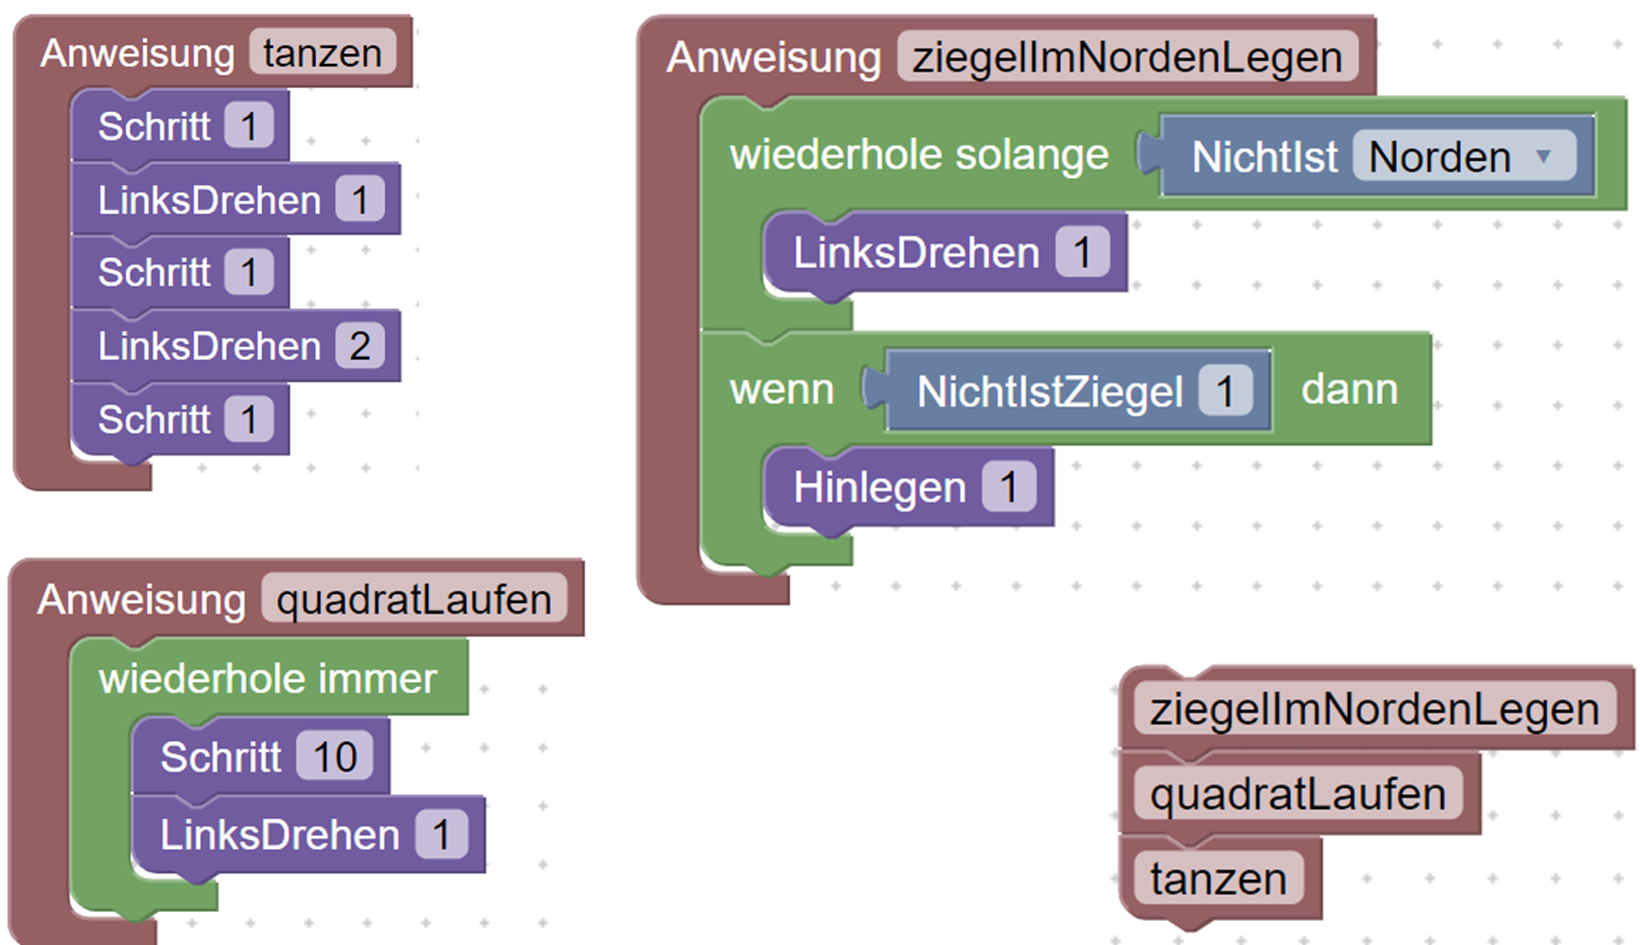
\includegraphics[width=0.75\textwidth]{_Aufgaben/BlocklyJava_Skript/img/A03_transMethods.png}
\end{center}


\LoesungKaro{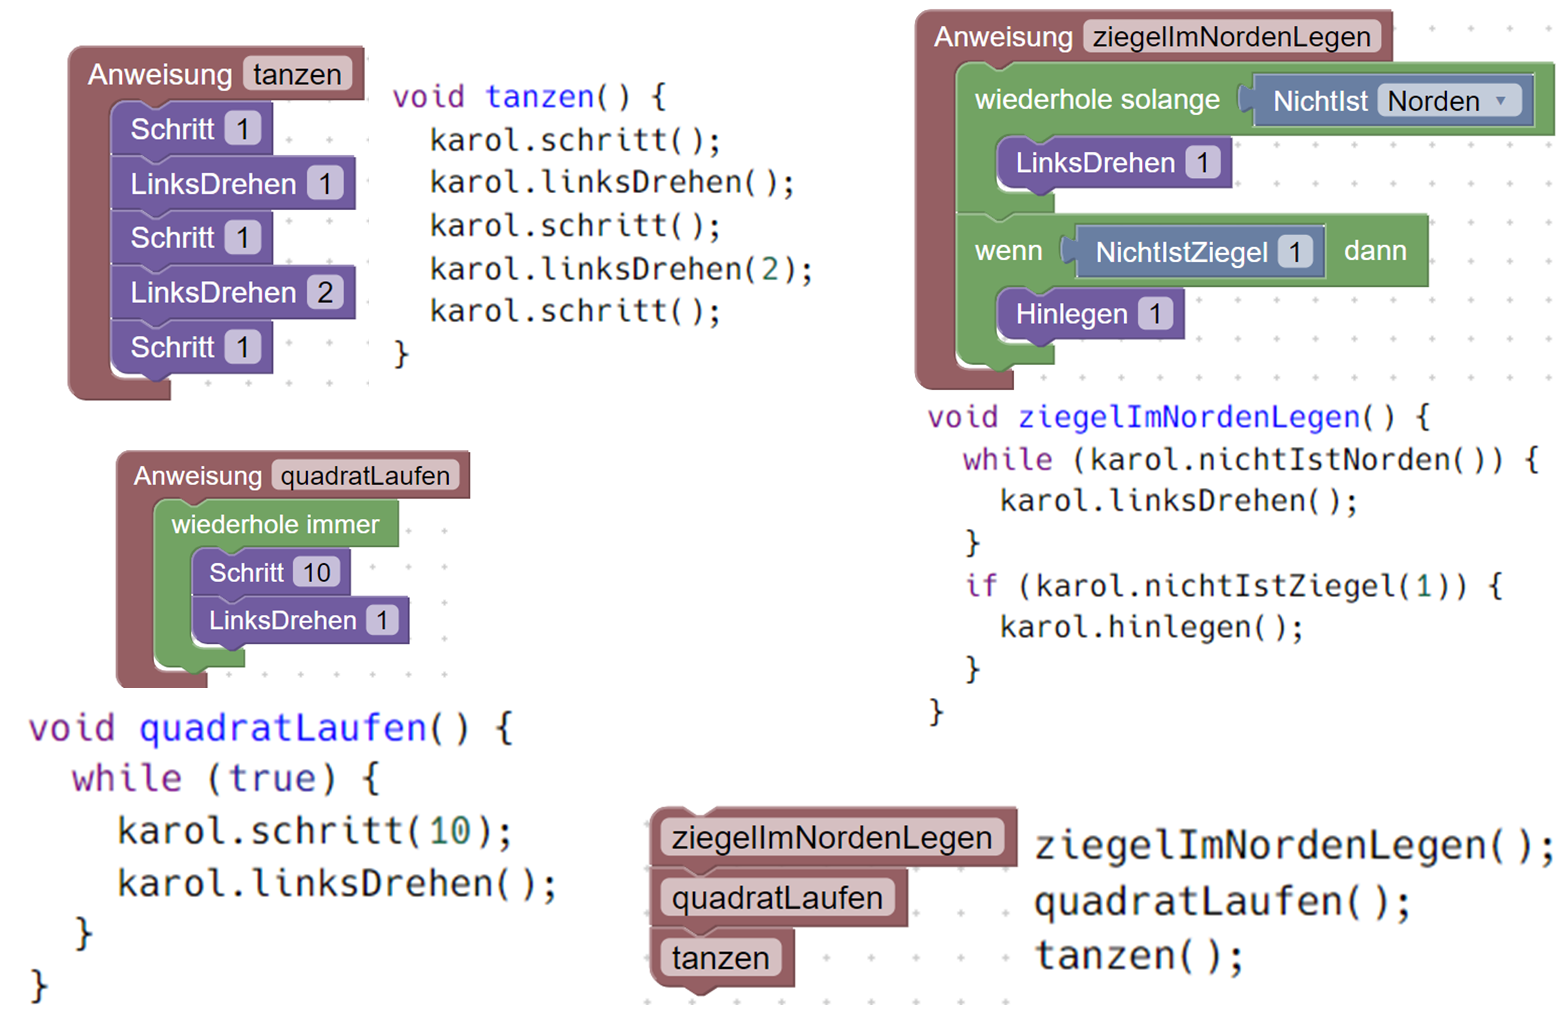
\includegraphics[width=\textwidth]{_Aufgaben/BlocklyJava_Skript/img/A03_transMethods_sol.png}}{32}
}

\Aufgabe{Karol mit Java und Struktogramme}

\doppelseite{0.55}{0.3}{t}{%
\begin{itemize}
    \item Bearbeite die Robot Karol (\url{karol.arrrg.de}) Level erneut. Schreibe den Programmcode dieses Mal direkt in Java!\\
    Zur Erinnerung: Deinen Code schreibst du an der gelb markierten Stelle in der main-Methode.
    \item Zeige nach den Schritten jeweils das Struktogramm an und notiere auf einem \emphColB{Schmierzettel}, wie du die letzte Spalte in Hefteintrag \ref{sec:befehlsarten} befüllen würdest.
    \item Was passiert, wenn du dein Programm aus eigenen Methoden aufbaust? Wieso ist das so?
\end{itemize}

}{%
 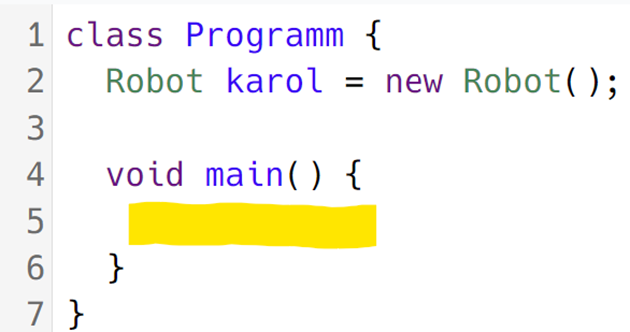
\includegraphics[width=\linewidth]{_Aufgaben/BlocklyJava_Skript/img/A04_karol_mainMarkiert.png}
 
 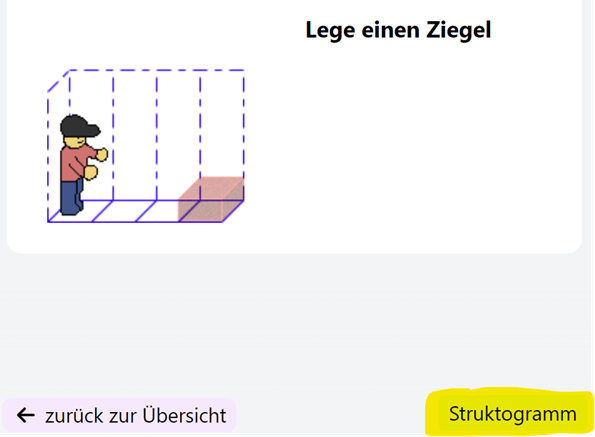
\includegraphics[width=\linewidth]{_Aufgaben/BlocklyJava_Skript/img/A04_karol_struktoMarkiert.png}
}



\Hefteintrag{2}{Programmablauf grafisch darstellen: Struktogramme}{%
Struktorgramme (auch: \LoesungLuecke{Nassi-Shneiderman-Diagramme}{12cm}) stellen \emphColA{Algorithmen (=Ablauf eines Programms)} grafisch dar. Ein Struktogramm bezieht sich immer auf genau eine Methode und stellt aufgerufene Methoden als ein Element dar.

In \textbf{Hefteintrag \ref{sec:befehlsarten}} sind die Struktogramm-Bausteine für verschiedene Befehlsarten dargestellt, die beliebig miteinander kombiniert werden können. 

Zusätzlich gibt es folgenden Baustein, der eine leere Stelle (z.B. leerer else-Block) darstellt:

\vspace{4cm}


}

\Aufgabe{Struktogramm-Training}{

Zeichne zu den folgenden Code Snippets jeweils ein Struktogramm:

\begin{center}
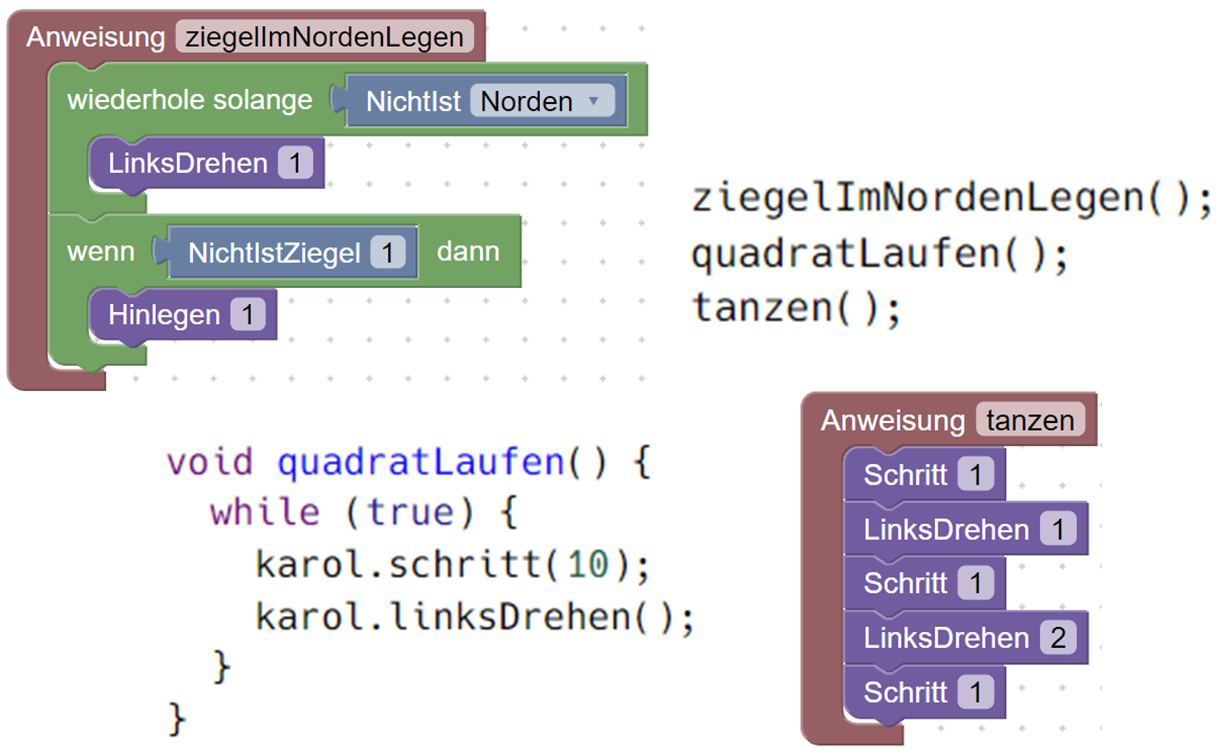
\includegraphics[width=0.75\textwidth]{_Aufgaben/BlocklyJava_Skript/img/A05_transMethods_strukto.png}
\end{center}


\LoesungKaro{}{29}
}

\Aufgabe{Neues Projekt mit BlueJ-Blockly}

1. BlueJ öffnen, neues Projekt erstellen, mit 'Choose' einen Speicherort auswählen und Namen eingeben. Immer auf Laufwerk H:/ speichern!
\\\\

\includegraphics[width=0.15\textwidth]{Aufgaben/BlocksAndJava/img/0_bluej.png} \hfill

\includegraphics[width=0.4\textwidth]{Aufgaben/BlocksAndJava/img/1_newProject.png} \hfill

\includegraphics[width=0.4\textwidth]{Aufgaben/BlocksAndJava/img/2_projectName.png}

\vspace{0.4cm}
2. Neue Klasse erstellen und per Rechtsklick mit Blockly öffnen.


\includegraphics[width=0.4\textwidth]{Aufgaben/BlocksAndJava/img/3_newClass.png} \hspace{0.5cm}

\includegraphics[width=0.25\textwidth]{Aufgaben/BlocksAndJava/img/4_blockly.png}

\vspace{0.4cm}
3. In Blockly (Fenster falls nötig in Taskleiste anklicken) neuen Methodenblock einfügen und falls benötigt Parameter (= input) über das Zahnrad hinzufügen. Parameter könne über Variablen verwendet werden.


\includegraphics[width=0.3\textwidth]{Aufgaben/BlocksAndJava/img/5_createParams.png} \hspace{0.5cm}

\includegraphics[width=0.3\textwidth]{Aufgaben/BlocksAndJava/img/6_variables.png}

\vspace{0.4cm}
4. In BlueJ die Klasse übersetzen/compilen, neues Objekt (mit beliebigem Namen) erzeugen und mit Rechtsklick auf das Objekt Methode aufrufen.

\centering

\includegraphics[width=0.25\textwidth]{Aufgaben/BlocksAndJava/img/7_compile.png} \hfill

\includegraphics[width=0.25\textwidth]{Aufgaben/BlocksAndJava/img/8_newObject.png} \hfill

\includegraphics[width=0.4\textwidth]{Aufgaben/BlocksAndJava/img/9_runMethod.png}

\input{_Aufgaben/BlocksAndJava/Methoden}

\Hefteintrag{2}{Methodenköpfe}{%

Im \LoesungLuecke{Methodenkopf}{8cm} können neben dem Namen noch weitere Informationen nach folgendem Schema gespeichert werden: 

\emphColB{Zugriffsmodifizierer} \emphColA{Rückgabetyp} \emphColC{name}(\emphColA{Datentyp} \emphColC{parametername}) \{ //... \}


\emphColB{public} \emphColA{void} \emphColC{schritteLaufen}(\emphColA{int} \emphColC{anzahl}, ...) \{ //... \}

\vspace{0.5cm}

Methodenname und Parametername können weitgehend frei gewählt werden (Groß- und Kleinschreibung beachten!). Folgendes ist \textbf{nicht} erlaubt:
\LoesungLine{Leerzeichen im Namen, Zahlen am Anfang des Namens, Rechenzeichen im Namen, Schlüsselwörter als Name}{3}

\vspace{0.5cm}

Die verwendeten \LoesungLuecke{Schlüsselwörter}{8cm} haben folgende Bedeutungen:

\emphColB{Zugriffsmodifizierer: public} - Methode kann ‚überall‘ verwendet werden. (im Gegensatz dazu \emph{private}: nur in der gleichen Klasse)

\emphColA{Datentyp} - Art der Daten (z.B. Ganzzahlen: \LoesungLuecke{int}{2cm}, Kommazahlen: \LoesungLuecke{double}{3cm}, Text: \LoesungLuecke{String}{3cm}, Wahrheitswert: \LoesungLuecke{boolean}{4cm})

\emphColA{Rückgabetyp} - Datentyp des Rückgabewerts (=\LoesungLuecke{return-value}{7cm}). Kann z.B. Ergebnis einer Berechnung sein. 

\emph{Besonderer Rückgabetyp} - \emph{void} bedeutet, die Methode hat keinen Rückgabewert. Außer bei void wird immer eine return-Anweisung benötigt.

\textbf{Parameter} - Speichert bei jedem Aufruf einen neuen Wert, der im Methodenrumpf über den Namen verwendet werden kann.


}

\Hefteintrag{2}{Methoden im Klassendiagramm}{%

\doppelseite{0.42}{0.52}{t}{%
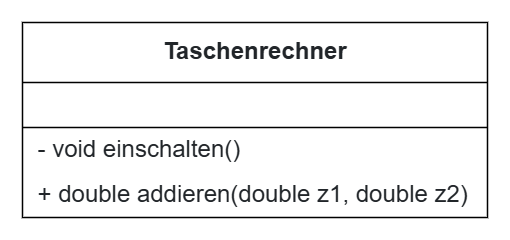
\includegraphics[width=\linewidth]{_Aufgaben//BlocklyJava_Skript//img/H07_KD.png}
}{%
    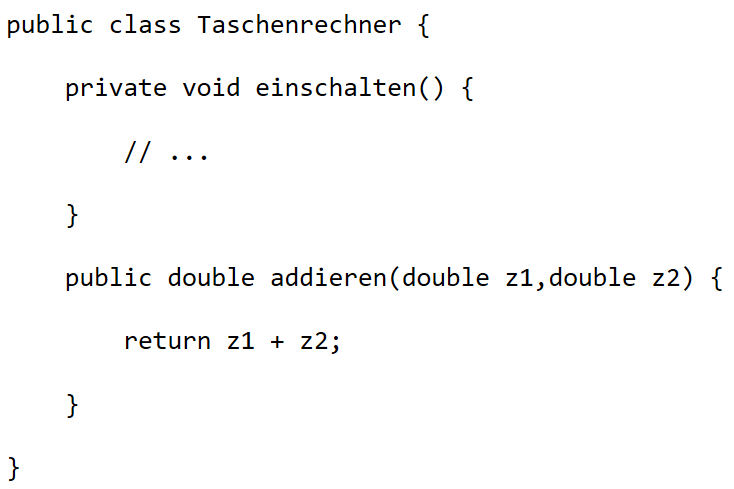
\includegraphics[width=\linewidth]{_Aufgaben//BlocklyJava_Skript//img/H07_Code.png}
}
}


\Aufgabe{Attribute im Klassendiagramm}{

Findet heraus, wie Attrbiute im Klassendiagramm dargestellt werden. Achtet auf \emphColB{Zugriffsmodifizierer, Datentyp und Name}. Macht eine Skizze auf einem Schmierblatt.

}

\Hefteintrag{2}{Attribute im Klassendiagramm}{%
Attribute werden im Klassendiagramm folgendermaßen dargestellt:

\centering
\vspace{1cm}
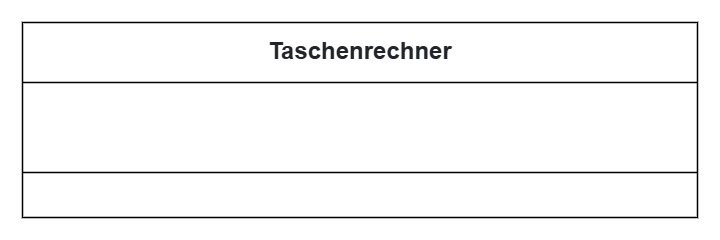
\includegraphics[width=0.7\textwidth]{_Aufgaben/BlocklyJava_Skript/img/H08_KD.png}


\vspace{1cm}

}


\begin{minipage}[t]{\textwidth}
\Aufgabe{Struktogramme und Klassendiagramme}

\textbf{Setze folgende Diagramme in BlueJ-Blockly um und notiere den Programmcode auf der nächsten Seite}

\vspace{0.5cm}

\doppelseite{0.45}{0.5}{t}{%
\textbf{Klassendiagramm:}

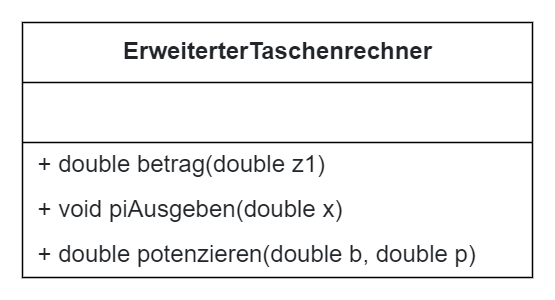
\includegraphics[width=\linewidth]{_Aufgaben/BlocksAndJava/img/klasse.png} 
}{%

\textbf{Struktogramm für piAusgeben(double x):}

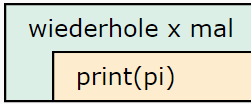
\includegraphics[width=0.6\linewidth]{_Aufgaben/BlocksAndJava/img/strukt_10pi.png}
}

\vspace{1cm}

\textbf{Zeichne hier die Struktogramme für die restlichen Methoden:}

\LoesungKaro{\\
\Large
+ double betrag(double z1) \\
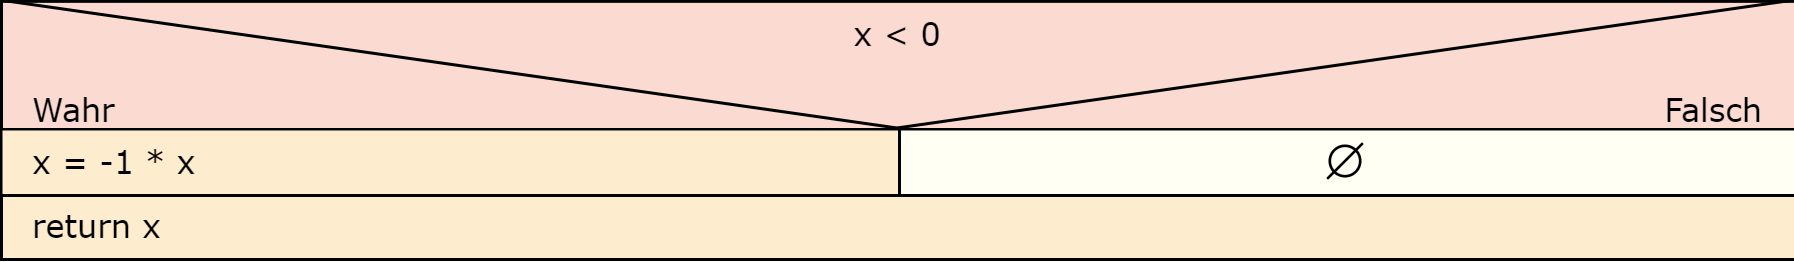
\includegraphics[width=\textwidth]{_Aufgaben/BlocksAndJava/img/strukt_betrag.png} \\\\
+ double potenzieren(double b, double p) \\
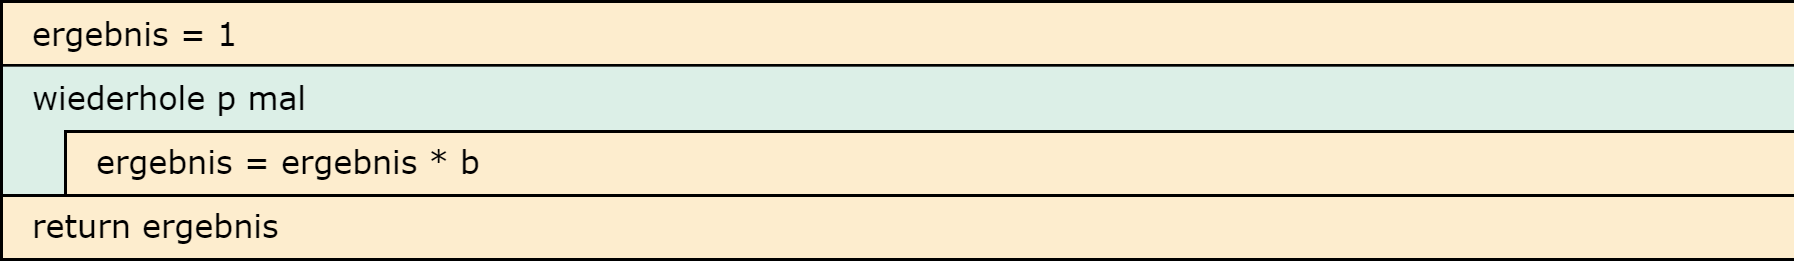
\includegraphics[width=\textwidth]{_Aufgaben/BlocksAndJava/img/strukt_protenz.png}}{25}

    
\end{minipage}


\begin{minipage}[t]{\textwidth}
\Large
\begin{lstlisting}[escapechar=\&]
public class ErweiterterTaschenrechner
{    
    public & \LoesungLuecke{double betrag(double z1) \{ }{15cm} &
    
        & \LoesungLuecke{if(z1 < 0) \{ }{15cm} &
        
            & \LoesungLuecke{z1 = -1 * z1;}{15cm} &
            
        & \LoesungLuecke{\}}{15cm} &   
        
        & \LoesungLuecke{return z1;}{15cm} &   
    }
    public & \LoesungLuecke{void piAusgeben(double x) \{ }{15cm} &
    
        & \LoesungLuecke{for(int i=0; i < x; i++) \{ }{15cm} &
        
            & \LoesungLuecke{System.out.println(Math.PI);}{15cm} &
            
        & \LoesungLuecke{\}}{15cm} &
    }
    public & \LoesungLuecke{double potenzieren(double b, double p) \{ }{15cm} &

        & \LoesungLuecke{double ergebnis = 1.0;}{15cm} &
    
        & \LoesungLuecke{for(int i=0; i < p; i++) \{ }{15cm} &
        
            & \LoesungLuecke{ergebnis = ergebnis * b;}{15cm} &
            
        & \LoesungLuecke{\}}{15cm} &
            
        & \LoesungLuecke{return ergebnis;}{15cm} &
    }
}
\end{lstlisting}

\end{minipage}

\Hefteintrag{2}{Übersicht: Variablen}{%



\Large \emphColB{Wertzuweisung} \large mit Gleichheitszeichen \emph{von rechts nach links}.

Schema: \emph{name = Wert;}\\
Beispiel: \emph{alter = 14;}

\vspace{0.4cm}\Large \emphColA{Verwendung des Werts} \large mit Variablenname statt eines Werts

Beispiel 1: \emph{System.out.println(alter);} statt  \emph{System.out.println(14);}\\
Beispiel 2: \emph{alter = alter + 1;} statt \emph{alter = 14 + 1;}

\vspace{0.4cm}\Large \emphColC{Vergleich des Werts} \large mit \emph{< , <= , == , >= , > ,  != , name.equals(Wert)}

Beispiele: \emph{x == 5} (x \LoesungLuecke{ist gleich}{4cm} 5) , \emph{x != 5} (x \LoesungLuecke{ungleich}{4cm} 5) , \emph{text.equals("Hallo")}~(text \LoesungLuecke{ist "Hallo"}{4cm}),


\vspace{0.4cm}\Large \emphColB{Deklaration} \large = Erstellen einer Varibale und Festlegung ihrer Eigenschaften.

\vspace{0.4cm}\Large \emphColA{Arten von Variablen} \large in der objektorientierten Programmierung:
\begin{itemize}
    \item \LoesungLuecke{lokale Variable}{8cm} deklariert  mit \emph{\textbf{Datentyp name;}} in einem Code-Block und nur dort verfügbar.
    \item \LoesungLuecke{Parameter}{8cm} (manchmal auch: Input/Argument) deklariert  mit \emph{\textbf{(Datentyp name)}} in den Klammern des Methodenkopfs und nur in dieser Methode verfügbar. Wert wird bei jedem Aufruf neu festgelegt.
    \item \LoesungLuecke{Attribut}{8cm} deklariert am Anfang der Klasse mit \emph{\textbf{private~Datentyp~name;}} Verfügbar in der ganzen Klasse mit anderem Wert für jedes Objekt. Zur Unterscheidung von lokalen Variablen kann bei der Verwendung auch \emph{this.name} geschrieben werden.
\end{itemize}


}


\begin{minipage}[t]{\textwidth}
\Aufgabe{Ein einfaches Spiel - Aufbau des Spielfelds}

\large

Ziel in diesem Jahr wird es sein, dass alle ein eigenes Spiel programmieren. Wir beginnen nun, den Grundstein hierfür zu legen.

\vspace{0.2cm}

%%%%%%%%%%%%%%%%%%%%%%%%%%%%%%%%%%%%%%
 % FÜR NÄCHSTES MAL MODIFIZIEREN!!!
%%%%%%%%%%%%%%%%%%%%%%%%%%%%%%%%%%%%%%
 
Für unser Spiel benötigen wir 2 Klassen:
\begin{itemize}
    \item \emphColB{Spielfeld}: Enthält alle Spielfiguren und zeigt sie mit einem Bild an einer bestimmten Position an.
    \item \emphColB{Spieler}: Eine Spielfigur, die du später mit der Tastatur steuern kannst. 
\end{itemize}

\vspace{0.2cm}

Zur Bewegung des Spielers wird ein Koordinatensystem, ähnlich zu dem in Mathematik, verwendet. Es ist jedoch etwas anders. Findet folgendes (z.B. mit Google) heraus und zeichnet es unten in das Fenster mit dem Spielfeld ein:
\begin{itemize}
    \item Wie ist das Koordinatensystem ausgerichtet (insbesondere: Wo ist der Ursprung, welche x- und y-Werte haben die Ecken des Spielfelds)?
    \item Was ist eine Hitbox und wo verläuft der Rand der (angenommen rechteckigen) Hitbox des Spielers (hier als Auto im Bild)?
    \item An welchem Punkt genau sind die Koordinaten des Spielers?
\end{itemize}

\vspace{2cm}
\begin{center}
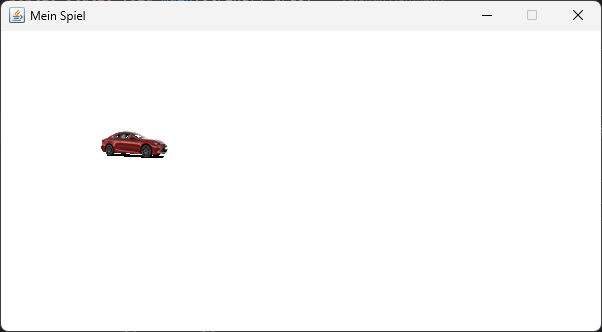
\includegraphics[width=0.9\linewidth]{_Aufgaben//BlocklyJava_Skript//img/A08_kosy.png}  
\end{center}

\vspace{2cm}

\end{minipage}



\normalsize
\begin{minipage}[t]{\textwidth}
\Aufgabe{Wo ist der Spieler?} 

Um auf dem Spielfeld angezeigt werden zu können, muss das Spielfeld 'wissen', was die Position und das Bild des Spielers sind. 

\begin{enumerate}
    \item Überlege, welche Attribute und Methoden die Klasse Spieler benötigt, damit die Spieler-Objekte auf dem Spielfeld angezeigt werden können. \\
	$\rightarrow$ Beachte hierbei, welche Zugriffsmodifizierer Attribute und Methoden haben!
     \item Die Bewegung eines Spieler-Objekts soll mit einer Methode \emph{run()} in der Klasse Spieler funktionieren, die vom Spielfeld immer wieder aufgerufen wird. 
	$\rightarrow$ \[schwer\] Welche Attribute und Methoden benötigt man noch, um hier später die Bewegung anhand der gedrückten Tasten programmieren zu können (angenommen, das Spielfeld-Objekt 'weiß' welche Tasten aktuell gedrückt sind)?
\end{enumerate}

Haltet eure Gedanken hier als Klassenkarte fest:

\LoesungKaro{}{30}

\end{minipage}

\Hefteintrag{1.9}{Besondere Methoden: Getter und Setter}{%


\doppelseite{0.38}{0.6}{t}{%

\Large \emphColA{Getter} \large haben den Zweck, den Wert eines (private) Attributs von anderen Klassen aus zugänglich zu machen. Der Methodenkopf folgt diesem Schema: 

\textbf{public}~\emph{TypAttribut}~\textbf{get}\emph{NameAttribut}\textbf{()}

\vspace{0.5cm}

\Large \emphColA{Setter} \large ermöglichen das Setzen von Attributwerten von außerhalb derselben Klasse. Sie haben einen Parameter mit dem Datentyp des Attributs und Rückgabetyp void. Der Methodenkopf folgt diesem Schema:


}{%
    %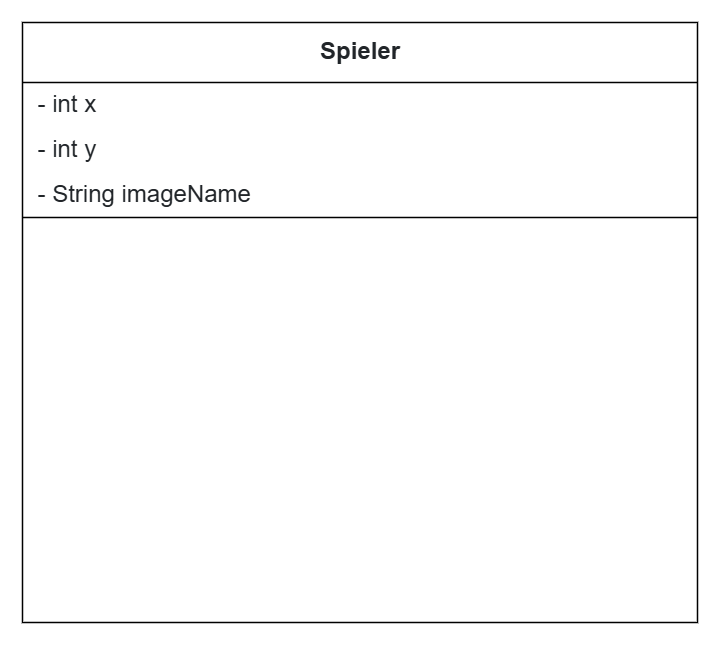
\includegraphics[width=1\linewidth]{_Aufgaben//BlocklyJava_Skript//img/H10_GetterSetter.png}

\begin{tikzpicture}
\begin{class}[text width=0.98\linewidth]{Spieler}{0 ,0}
\attribute{- int x}
\attribute{- int y}
\attribute{- String imagePath}
\operation{}
\operation{}
\operation{}
\operation{}
\operation{}
\operation{}
\operation{}
\operation{}
\end{class}
\end{tikzpicture}
}

\textbf{public void set}\emph{NameAttribut}\textbf{(}\emph{TypAttribut}~\textbf{wert)}\\

\Large \emphColA{Standard-Getter/-Setter} \large lesen bzw. schreiben den Wert des Attributs direkt (ohne Prüfung). Allgemein können Setter vor dem Schreiben den Parameter auf Gültigkeit prüfen oder modifizieren. 
}


\Aufgabe{Spiel-Vorlage und erster Start}

\begin{itemize}
    \item Kopiere den \textbf{ganzen Ordner} SpielProjekt vom Ressourcen-Laufwerk in euren Ordner H:\\  \emph{R:/gy0187/klassen/gy0187-klasse-9b/Vorlagen/SpielProjekt}
    \item Öffne die Datei \emph{package.bluej} (manchmal heißt sie auch nur \emph{package}) in deiner Kopie der Vorlage.
    \item War das erfolgreich, kannst du ein Spielfeld-Objekt und ein Spieler-Objekt erstellen, das Spielerobjekt zum Spielfeld hinzufügen und das Spiel starten (siehe Bilder unten).
\end{itemize}

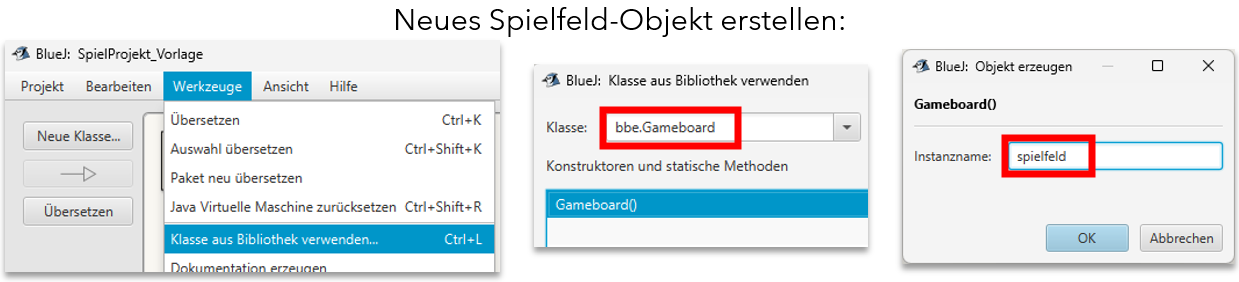
\includegraphics[width =\textwidth]{_Aufgaben/BlocklyJava_Skript/img/A10_CreateGB.png}

\vspace{0.2cm}
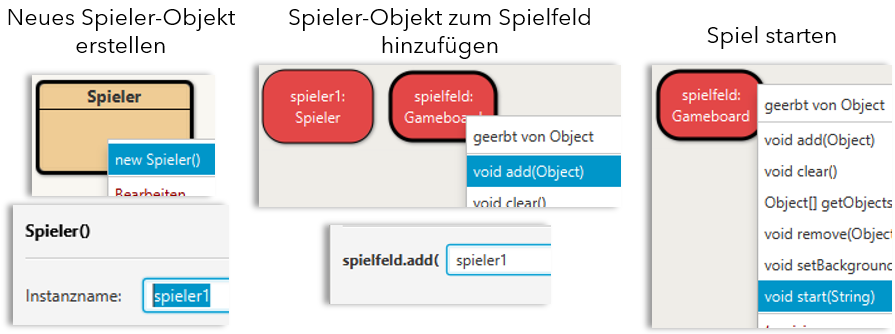
\includegraphics[width=\textwidth]{_Aufgaben/BlocklyJava_Skript/img/A10_StartGame.png}




\Aufgabe{Spieler programmieren}{
\begin{minipage}[t]{0.5\textwidth}
\normalsize
\vspace{-11cm}
    Probiere nach jedem Schritt aus, was passiert, wenn du dein Spiel startest!
    \begin{enumerate}
        \item Programmiere die Klasse Spieler wie im Klassendiagramm
        vorgegeben. Programmiere getX() und getY() als Standard-Getter, lasse
        act() erstmal leer.
        \item Erstelle einen Konstruktor und setze dort die Koordinaten
        auf feste Werte und finde damit heraus, wie groß das
        Spielfeld ist. Hierfür musst du etwas herumprobieren.
        \item Notiere den Programmcode von getX() und getY() auf der
        nächsten Seite.
        \item Das Spielfeld führt die Methode act() seiner Spieler-Objekte
        ca. 25x pro Sekunde aus. Finde heraus, wie du damit ein
        Spieler-Objekt auf dem Spielfeld bewegen kannst.
        \item Wie kann man die Bewegungsgeschwindigkeit des Spiel-
        ers festlegen? Probiere deine Idee im Programm aus und
        ergänze das Klassendiagramm und den Programmcode auf
        der nächsten Seite.
        \item Wie kann man zu Beginn des Spiels die Startposition des
        Spielers (bei jedem neuen Objekt woanders) festlegen? Pro-
        biere auch das wieder aus und ergänze das Klassendia-
        gramm.
        \item Über den Toolbox-Ordner `Grafik: Objekte` kannst du in der Main 
        weitere geometrische Formen hinzufügen. Nutze das, um ein kleines 
        Spiel zu programmieren.
    \end{enumerate}
\end{minipage}
\hfill
\begin{minipage}[t]{0.47\textwidth}
\large
%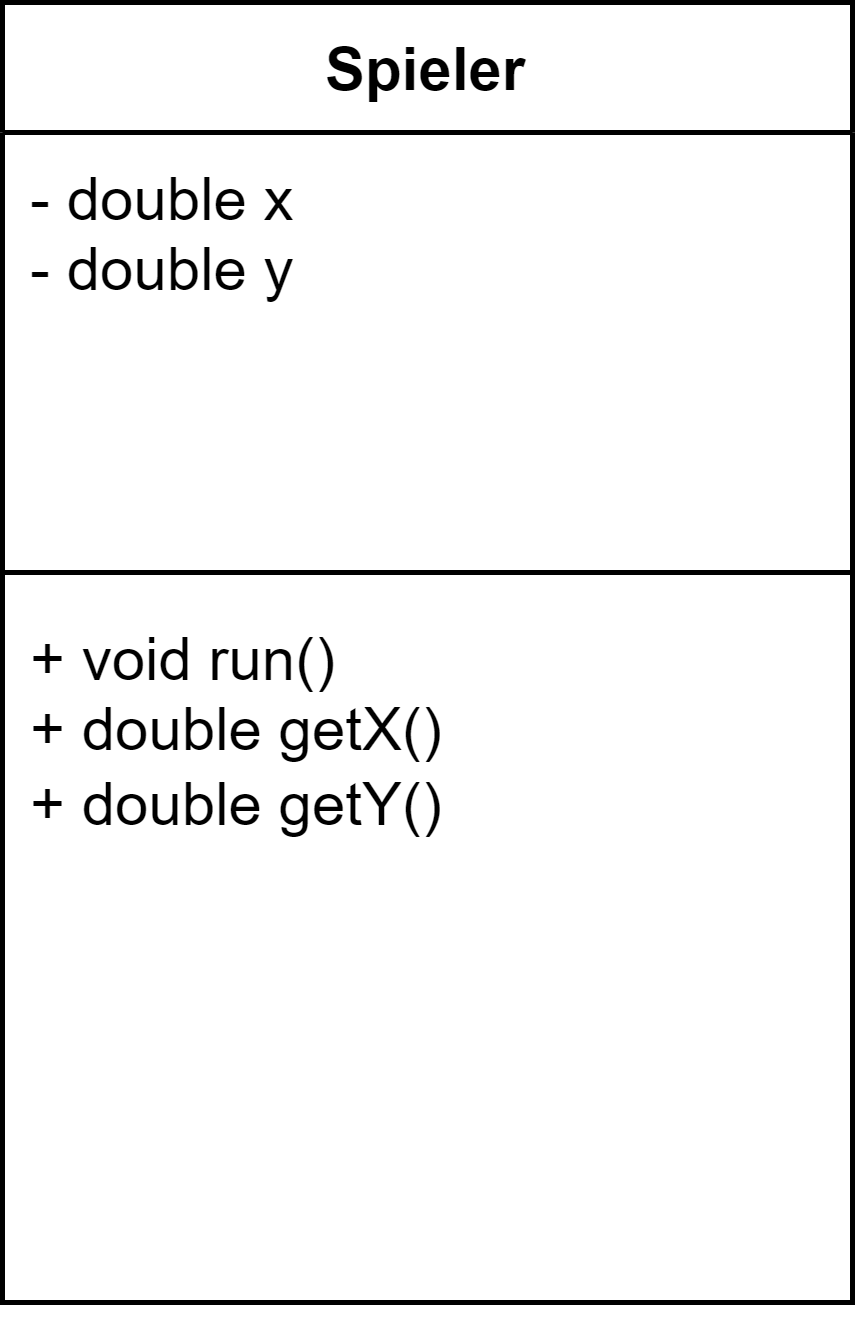
\includegraphics[width=0.9\linewidth]{_Aufgaben/BlocksAndJava/img/57_Klassendiagramm.png}
\begin{tikzpicture}
\begin{class}[text width=\linewidth]{Spieler}{0 ,0}
\attribute{- double x}
\attribute{- double y}
\attribute{}
\attribute{}
\attribute{}
\attribute{}
\attribute{}
\operation{+ void act()}
\operation{+ double getX()}
\operation{+ double getY()}
\operation{}
\operation{}
\operation{}
\operation{}
\operation{}
\operation{}
\operation{}
\operation{}
\operation{}
\operation{}
\operation{}
\end{class}
\end{tikzpicture}
\end{minipage}
}

\pagebreak

\large
\begin{lstlisting}
public class Spieler {
    private double x;
    private double y;

    (*@\LoesungLuecke{private double speedX;}{10cm}@*)

    (*@\LoesungLuecke{private double speedY;}{10cm}@*)
    
    public double getX() {
    
        (*@\LoesungLuecke{return x;}{10cm}@*)
    }
    public double getY() {
    
        (*@\LoesungLuecke{return y;}{10cm}@*)
    }
    public void act() {
    
        (*@\LoesungLuecke{x += speedX;}{10cm}@*)
        
        (*@\LoesungLuecke{y += speedY;}{10cm}@*)
        
        (*@\LoesungLuecke{y += speedY;}{10cm}@*)
        
        (*@\LoesungLuecke{y += speedY;}{10cm}@*)
        
        (*@\LoesungLuecke{y += speedY;}{10cm}@*)
    }
    
    public void (*@\LoesungLuecke{setX(double wert}{10cm}@*) {
    
        (*@\LoesungLuecke{x = wert;}{10cm}@*)
    }
    
    public void (*@\LoesungLuecke{setY(double wert}{10cm}@*) {
    
        (*@\LoesungLuecke{y = wert;}{10cm}@*)
    }
    
    public (*@\LoesungLuecke{Spieler(double startX, double startY}{10cm}@*) {
    
        (*@\LoesungLuecke{x = wert;}{15cm}@*)
        
        (*@\LoesungLuecke{y = wert;}{15cm}@*)
    }
}
\end{lstlisting}

\Hefteintrag{1.5}{Besondere Methoden: Konstruktoren}{%
Konstruktoren sind spezielle Methoden, die genutzt werden, um ein \emphColA{Objekt zu initialisieren/konstruieren}. Ein Konstruktor wird \emphColA{automatisch beim Erstellen eines Objekts} aufgerufen. 

In Java erkennt man einen Konstruktor insb. an zwei Dingen:
\begin{enumerate}
    \item Er \emphColA{heißt} \emphColA{\LoesungLuecke{genauso wie die Klasse}{12cm}}.
    \item Er hat \emphColA{keinen \LoesungLuecke{Rückgabetyp}{8cm}}.
\end{enumerate}

Ansonsten verhält er sich wie eine Methode und kann z.B. Parameter haben, die dann oft als Startwerte für das Objekt dienen.

Ein typischer Konstruktor im Programmcode sieht z.B. so aus: \\
\emphColB{public Spieler(double startX , double startY) \{ \\ 
~~~~~~x = startX;\\
~~~~~~y = startY;\\
\}}

Im Klassendiagramm würde dieses Beispiel so eingetragen:

\vspace{0.2cm}

\emphColB{\LoesungLuecke{+ Spieler(double startX, double startY)}{12cm}}




Ein neues Objekt erstellt und speichert man dann z.B. so: \emph{Spieler s1 = new Spieler(100,50);}




}

\Hefteintrag{1.3}{Besondere Methoden: Main/Hauptprogramm}{%
Möchte man für ein Java-Programm starten, benötigt man eine \emphColA{\LoesungLuecke{main-Methode}{8cm}}.

Diese nennt man auch den \emphColA{Einstiegspunkt/Hauptprogramm} eines Programms. In ihr werden meistens die benötigten \LoesungLuecke{Objekt}{5cm} erstellt und ihre \LoesungLuecke{Methoden}{5cm} aufgerufen.

Der \emphColC{Kopf} der Main-Methode ist immer gleich (siehe Bsp.):

\emphColC{public static void main() \{}\\
~~~~~~\emph{Spieler s1 = new Spieler(100,50);}\\
~~~~~~\emph{// ... weitere Objekte und Methoden}\\
\emphColC{\}}

Das Schlüsselwort \LoesungLuecke{static}{3cm} bedeutet hierbei, dass kein Objekt benötigt wird, um die Methode aufzurufen. In Blockly2Java wird die main-Methode automatisch zum Ausführen ausgewählt.
}




\Aufgabe{Gameboard-Library}

\doppelseite{0.47}{0.47}{t}
{%
Die Gameboard Library stellt im package \emph{bbe} ein fertiges \emph{Gameboard} zur Verfügung, zu dem Objekte (so genannte Entities) hinzugefügt werden können. Zur Festlegung der Darstellung der Entities können (aber müssen nicht!) verschiedene Methoden implementiert werden, die rechts in der Klasse \emph{ExampleEntity} dargestellt werden.

Weitere Informationen zu den Methoden gibt es im Struktogramm auf der nächsten Seite und unter \href{https://gameboard.valentin-herrmann.com}{gameboard.valentin-herrmann.com}

\vspace{0.5cm}
\begin{tikzpicture}
\begin{class}[text width=\linewidth]{Gameboard}{0 ,0}

\operation{+ Gameboard()}
\operation{+ void add(Object obj)}
\operation{+ void remove(Object obj)}
\operation{+ void clear()}
\operation{+ void start(String title)}
\operation{+ void setBackgroundImagePath(String path)}
\operation{+ void setShowHitboxes(boolean show)}
\operation{+ Object[] getObjects()}

\end{class}
\end{tikzpicture}
}
{%
\begin{tikzpicture}
\begin{class}[text width=\linewidth]{ExampleEntity}{10 ,0}

\operation{+ Number getX()}
\operation{+ Number getY()}
\operation{+ String getText()}
\operation{+ String getImagePath()}
\operation{+ double getScaleFactor()}
\operation{+ boolean isStatic()}
\operation{+ String getGameoverMessage()}
\operation{}
\operation{+ void setLeft(boolean pressed)}
\operation{+ void setRight(boolean pressed)}
\operation{+ void setUp(boolean pressed)}
\operation{+ void setDown(boolean pressed)}
\operation{+ void setW(boolean pressed)}
\operation{+ void setA(boolean pressed)}
\operation{+ void setS(boolean pressed)}
\operation{+ void setD(boolean pressed)}
\operation{+ void setEnter(boolean pressed)}
\operation{+ void setSpace(boolean pressed)}
\operation{}
\operation{+ void crash()}
\operation{+ void crash(String className)}
\operation{+ void crash(Object other)}
\operation{+ void crash(String className, Object other)}


\end{class}
\end{tikzpicture}
}

\vspace{0.5cm}

\textbf{Gameboard in der Main-Methode erzeugen:}

\normalsize
\begin{verbatim}
import bbe.Gameboard;                     // Gameboard Library importieren
public static void main(String[] args) {  // Methodenkopf von main
   Spieler spieler1 = new Spieler();      // Spieler erstellen
   Gameboard spiefeld = new Gameboard();  // Gameboard erstellen
   spielfeld.add(spieler1);               // Spieler zum Gameboard hinzufügen
   spielfeld.start("Spiel");              // Spiel mit Fenstertitel "Spiel" starten
}
\end{verbatim}

\large
\textbf{Gameboard in BlueJ graphisch erzeugen:}

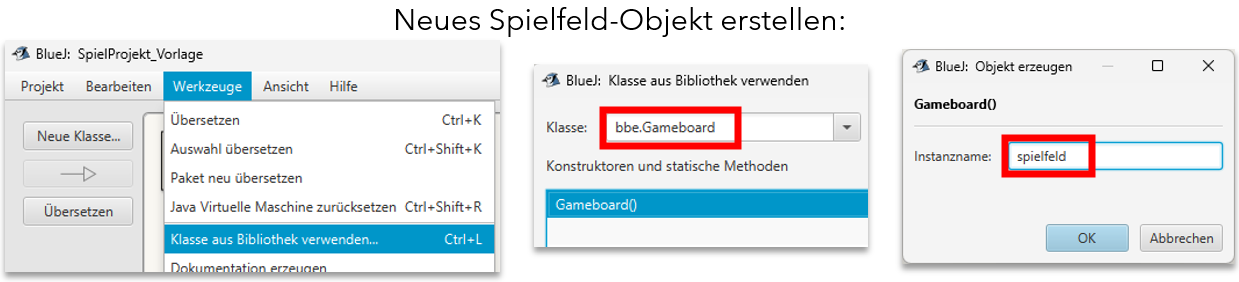
\includegraphics[width =\textwidth]{_Aufgaben/BlocklyJava_Skript/img/A10_CreateGB.png}



\begin{minipage}{\textwidth}
\subsection*{Interner Ablauf des Gameboards}

Dieses Struktogramm stellt den internen Ablauf des Gameboards beim Ausführen des Spiels dar. 

\fbox{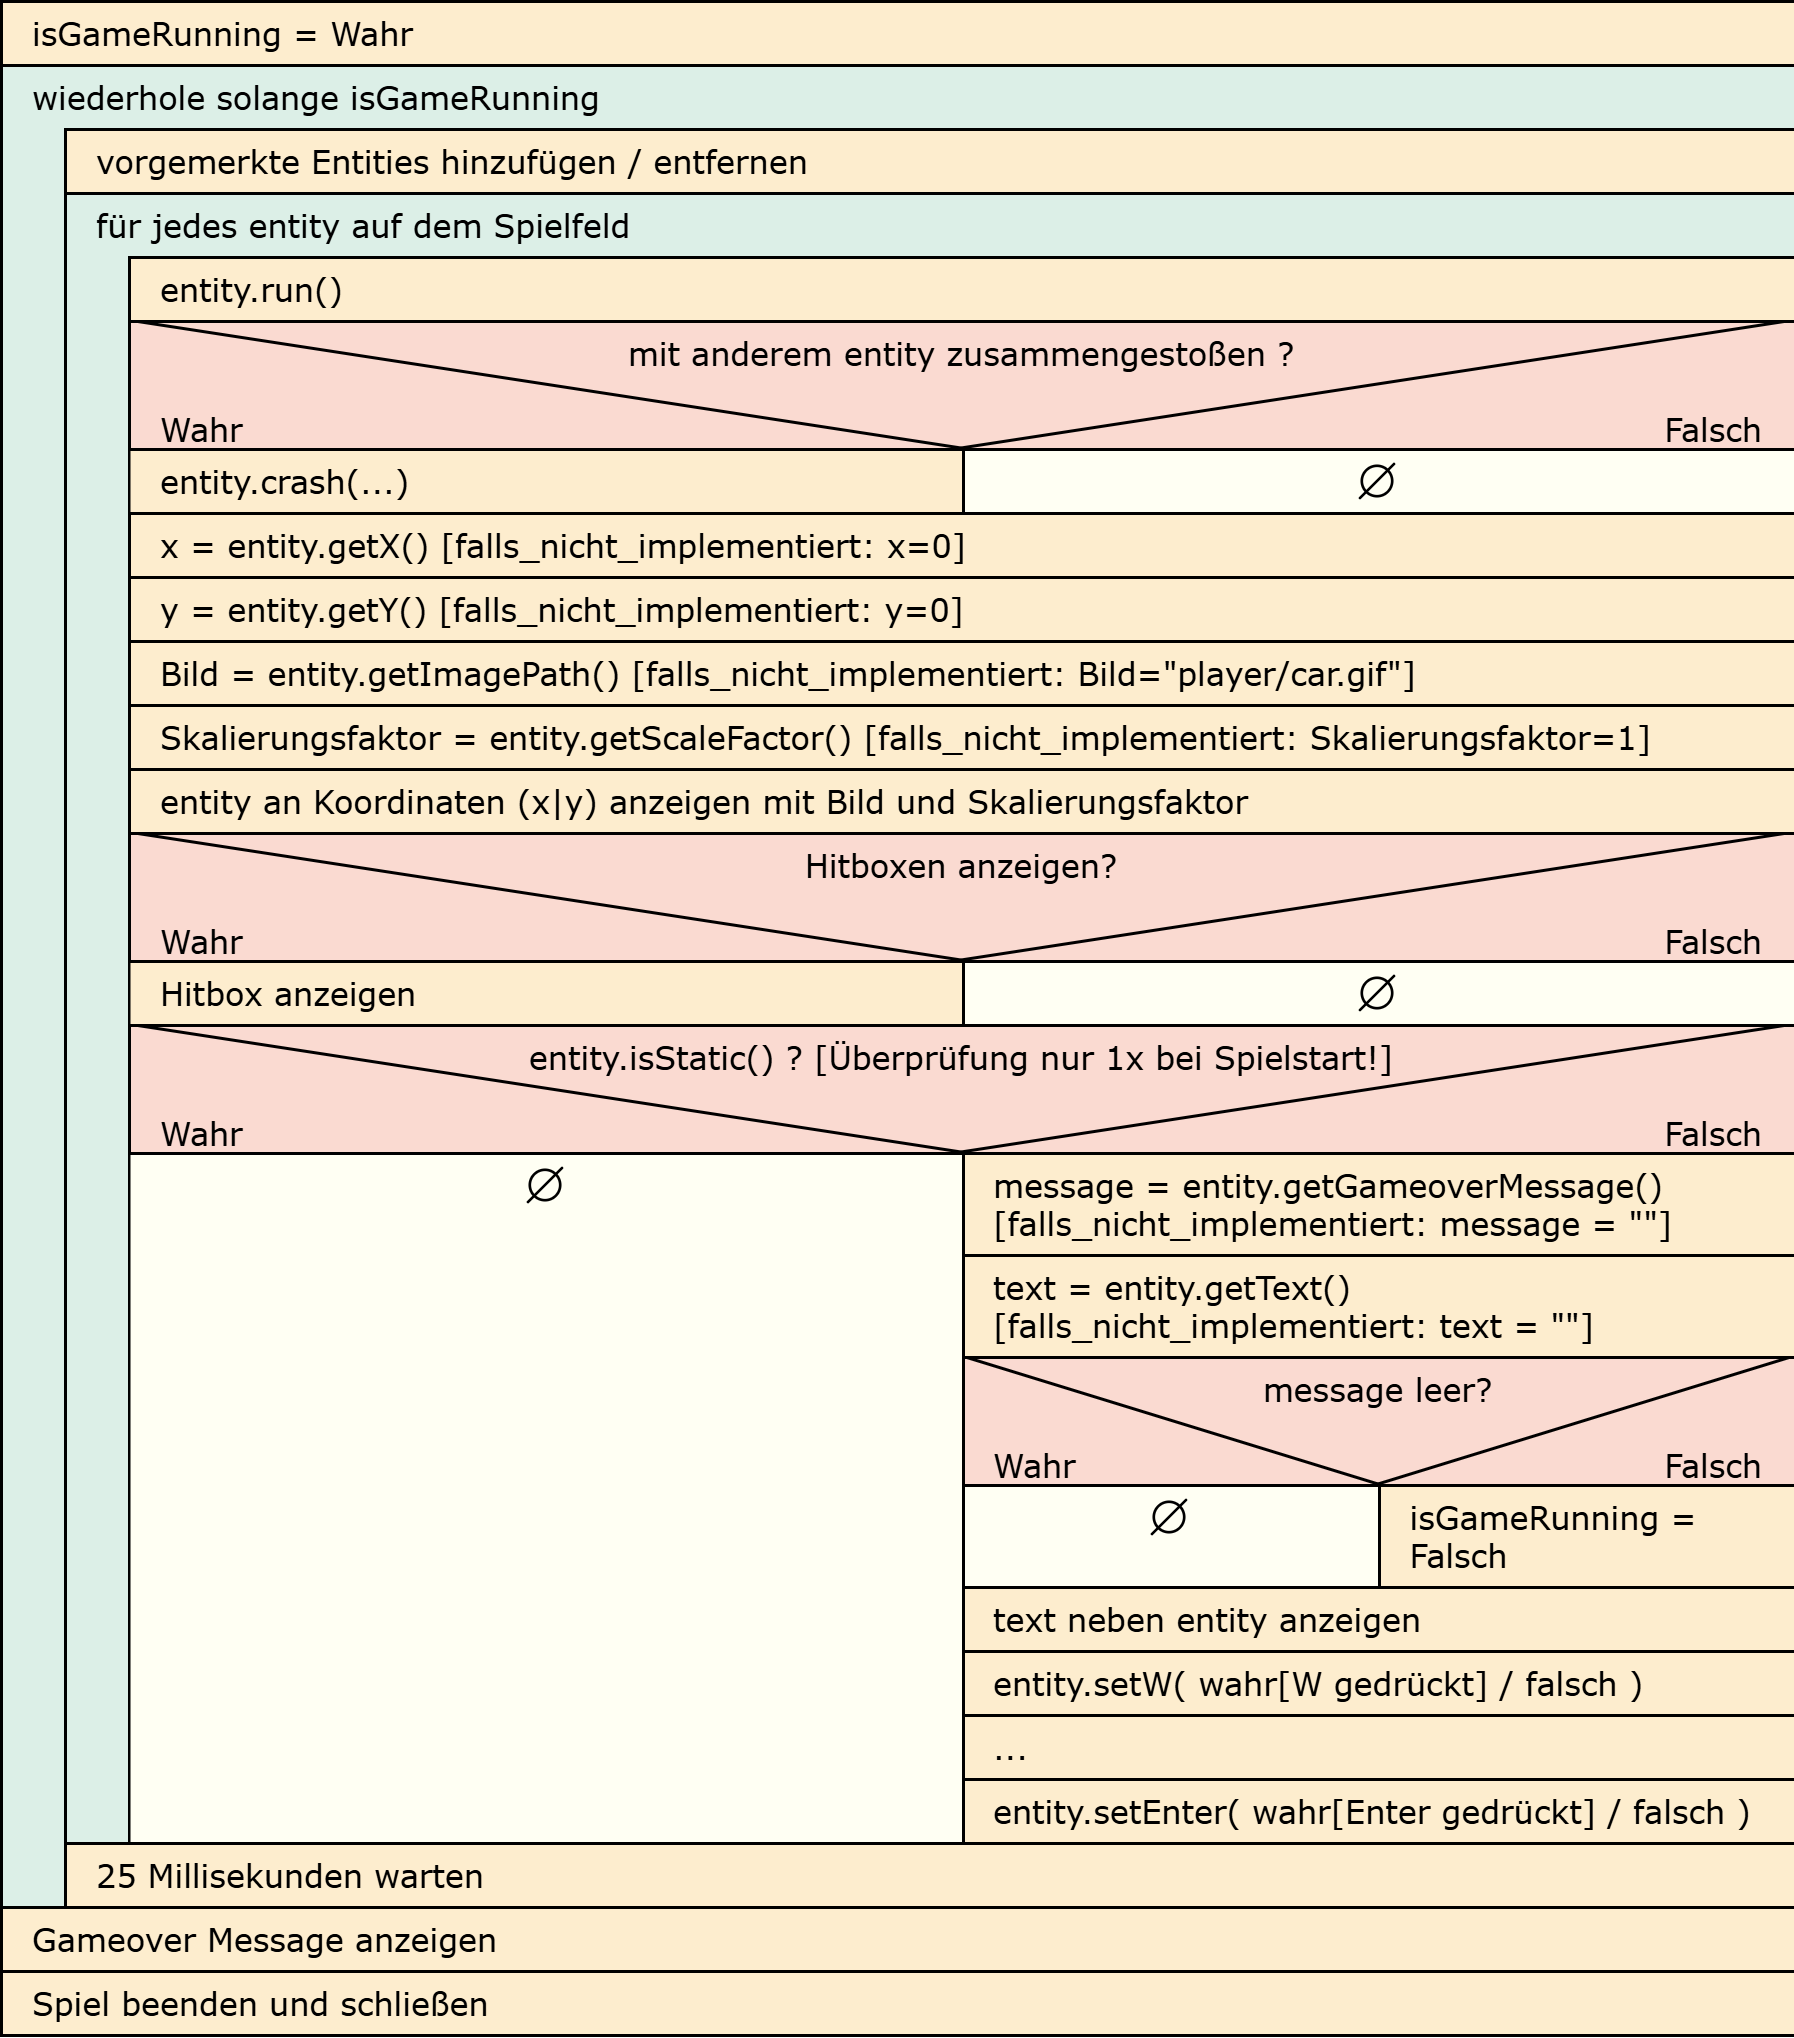
\includegraphics[width=\textwidth]{_Aufgaben/BlocklyJava_Skript/img/P_struktog_Gameboard.png}}
    
\end{minipage}